\documentclass[11pt]{article}
\usepackage{amsmath, amssymb, amsthm} 
\usepackage[spaces, hyphens]{url}
\usepackage{hyperref}
\usepackage{booktabs}
\usepackage{multirow}
\usepackage{graphicx}
\usepackage{float}

\usepackage[letterpaper, top=1in, bottom=1in, left=1in, right=1in, heightrounded]{geometry}

\setlength{\parindent}{0pt}
\setlength{\parskip}{0.6em}

\title{\vspace{-1.5em}Evaluating Randomised Algorithms and Their LLM Generated Counterparts on the Bin Packing Problem\vspace{-0.5em}}
\author{Joshua Raybould}
\date{}
\begin{document}

\maketitle
\vspace{-2em}

\begin{abstract}
This report describes the design and evaluation of a diverse suite of human-implemented randomised algorithms for the one-dimensional offline Bin Packing Problem (BPP), and compares them against implementations generated from scratch by two state-of-the-art Large Language Models: OpenAI's GPT-5.2 and Anthropic's Claude Opus 4.6. Eight algorithms spanning simple heuristics, local search methods, and population-based metaheuristics were implemented, tuned, and benchmarked. An automated iterative refinement pipeline was used to generate LLM counterparts for each algorithm. Results show that LLMs can produce competitive and sometimes superior implementations for well-studied combinatorial problems, though they remain capable of subtle reasoning errors that pass correctness checks while undermining search effectiveness.
\footnote{A longer form report is available at \texttt{/docs/main.pdf} in the project repository.}
\end{abstract}

\section{Introduction}

\subsection{Problem Background and Definition}

The bin packing problem (BPP) is a central problem in combinatorial optimisation. In its standard one-dimensional (1D) formulation, a set of $n$ items with weights (or equivalently, sizes) $w_i$ must be packed into bins of uniform capacity $C$ such that the total number of bins used is minimised. This study focuses on the offline variant, where all item weights are known in advance. Beyond its theoretical significance, bin packing has numerous real-world applications, ranging from loading transport vehicles with weight capacities to minimising waste in industrial cutting processes \cite{munien}. Additionally, many scheduling problems contain the BPP as a special case.

Formally, we define binary variables $y_j = 1$ if bin $j$ is used and $0$ otherwise, and $x_{ij} = 1$ if item $i$ is assigned to bin $j$ and $0$ otherwise, with $u$ as an upper bound on the number of bins \cite{maxence}. The objective is:
$$\min\sum_{j=1}^{u} y_j,$$
subject to each item being packed exactly once and no bin exceeding capacity $C$:
$$\sum_{j=1}^{u} x_{ij} = 1, \;\; \forall i \qquad \sum_{i=1}^{n} x_{ij} w_{i} \leq C y_j, \;\; \forall j.$$

The 1D offline BPP is strongly NP-hard, established via a polynomial-time reduction from the 3-Partition problem \cite{garey}. As a consequence, no polynomial-time algorithm for solving the BPP to optimality is known, assuming P $\neq$ NP. For large-scale instances, approximation algorithms and stochastic metaheuristics that trade guaranteed optimality for computational efficiency are therefore necessary.

\subsection{Literature Review}

The 1D BPP has been studied extensively for many decades. Exact methods, including branch-and-bound and column generation, can solve instances to optimality but become intractable as instance size grows \cite{garey, maxence}. A widely used constructive heuristic is First Fit Decreasing (FFD); due to its strong baseline performance, it is commonly used to initialise more sophisticated methods. A broad range of metaheuristics have been applied to the BPP. These include Simulated Annealing with FFD initialisation and a sum-of-squares objective \cite{sonuc}, Variable Neighbourhood Search using a Minimum Bin Slack heuristic \cite{kryz}, the Grouping Genetic Algorithm (GGA) of Falkenauer \cite{gga}---extended in the GGA-CGT framework \cite{quirozca}, which uses a group-oriented encoding to prevent crossover from destroying well-packed structures---and Ant Colony Optimisation (ACO) adapted by Levine and Ducatelle \cite{levine}. While numerous studies compare subsets of these algorithms, comprehensive cross-paradigm empirical comparisons are much rarer \cite{munien}, motivating the baseline evaluation conducted in this study.

\subsection{Large Language Models and Code Generation}

LLMs trained on massive corpora of text and code have demonstrated strong code generation capabilities for well-represented tasks \cite{chang}. However, they struggle with tasks requiring genuine reasoning in novel scenarios \cite{kucharavy}; on LeetCode problems, correctness deteriorates sharply on newly released questions absent from training corpora \cite{coignion}, suggesting that performance conflates knowledge retrieval with genuine algorithmic synthesis.

A growing body of work examines LLMs in combinatorial optimisation specifically. ReEvo \cite{reevo} uses an evolutionary framework in which LLMs iteratively generate and refine heuristic components---such as the heuristic measure function that guides decisions within an ACO framework---frequently matching human-designed approaches. Rosin \cite{rosin2025} gives LLMs broader freedom to select and implement search strategies, demonstrating that generated code can resolve previously open combinatorial instances. In these cases, the LLM operates at the level of heuristic components or freely chooses the strategies. Our study instead tasks LLMs with producing complete implementations of named metaheuristics---including design decisions such as objective function selection and parameter selection---and directly compares the results against human-written baselines.

\subsection{Research Questions}

\begin{enumerate}
    \item How do various human-implemented randomised algorithms compare in empirical performance across diverse problem instances?
    \item How effective are flagship LLMs at producing functionally correct metaheuristic implementations that achieve competitive solution quality within a fixed time budget?
    \item To what degree does performance vary across different LLMs, and are there identifiable patterns or common shortcomings in their generated code?
\end{enumerate}

\section{Human-Implemented Metaheuristics}

To establish a robust empirical baseline, we implemented eight stochastic algorithms for the 1D BPP. Parameter values were selected through manual trial-and-error tuning on a set of uniform test instances (test-u: 10 instances of 400 items and 10 of 800 items), targeting an average execution time of approximately 20 seconds per run. All algorithms were designed, written, and tuned by the author with reference to the relevant literature, with LLMs consulted solely to identify bugs and oversights.

\subsection{Common Components}

All algorithms utilise the $L_2$ lower bound of Martello and Toth \cite{martello} as a strict stopping criterion, which provides a tighter bound than the trivial $\lceil \sum_{i=1}^{n} w_i / C \rceil$ by accounting for items that cannot share bins.

Solution fitness is evaluated using the sum-of-squares objective function, originally introduced by Falkenauer \cite{gga} and subsequently employed across a range of metaheuristic implementations \cite{sonuc, kryz}:
$$f = \sum_{j=1}^{u} \left( {\sum_{i=1}^{n} x_{ij} w_{i}} \right)^2.$$
In this formulation, the inner sum represents the total weight of the items packed into bin $j$, meaning the overall fitness evaluates the sum of the squared weights of all active bins. If the objective relied solely on the total number of active bins, it would remain unchanged for the vast majority of transitions — since a move only affects the bin count when it completely empties a bin — leaving the search with no signal to distinguish between neighbouring solutions \cite{gga}. The sum-of-squares formulation resolves this by yielding a higher fitness when items are concentrated into tightly packed bins, guiding the algorithm to starve lightly packed bins until they can be emptied entirely.

\subsection{Algorithm Descriptions}

\textbf{Randomised Best Fit (RBF).} The simplest baseline: items are randomly shuffled, then packed using standard Best Fit, which places each item into the bin with the smallest sufficient residual capacity. The random shuffle helps mitigate adversarial input orderings.

\textbf{Simulated Annealing (SA).} Simulated Annealing is a probabilistic local search metaheuristic. Like hill-climbing, it iteratively generates neighbouring solutions, but unlike hill-climbing it accepts worse solutions with a probability that decreases over time according to a temperature parameter. This allows the search to escape local optima early on, gradually focusing on exploitation as the temperature cools \cite{gendreau}.

Our implementation is inspired by Sonu\c{c} et al.\ \cite{sonuc} and initialises with FFD. Neighbours are generated by selecting two distinct bins at random and either moving a single random item from one to the other or swapping two items between them, with equal probability. Infeasible moves that would violate a bin's capacity constraint are rejected outright without performing a temperature update or acceptance calculation. The fitness change is normalised by the bin capacity to help with scaling. We set $T_0 = 20{,}000$ with exponential cooling $\alpha = 0.9996$, terminating when $T \leq 0.01$.

\textbf{Tabu Search (TS).} Tabu Search is a local search metaheuristic that extends hill-climbing by maintaining a short-term memory of recently visited configurations. By forbidding the algorithm from returning to these for a set number of iterations, it is forced past local optima into unexplored regions of the search space \cite{gendreau}.

Our implementation initialises with FFD and evaluates fitness using the sum-of-squares objective. During each of 18,500 iterations, 35 candidate moves are generated: each selects two random bins and either swaps two items or moves a single item. To aggressively reduce the bin count, a targeted heuristic inspired by Lodi et al.\ \cite{lodi} selects the least full bin as the move source with 60\% probability, actively guiding the search toward emptying bins entirely. The best valid neighbour is selected each step, even if it worsens fitness. A tabu list of 4 recent moves prevents cycling, and an aspiration criterion overrides tabu status when a move eliminates a bin entirely, as this guarantees a strict improvement to the global objective.

\textbf{Variable Neighbourhood Search (VNS).} VNS is a metaheuristic that escapes local optima by progressively widening its perturbation when the search stagnates \cite{gendreau}. Starting with $k = 1$, the current solution is perturbed by applying $k$ random moves (shaking), then locally optimised. If the result improves the incumbent solution, $k$ resets to 1; otherwise $k$ is incremented, producing a stronger perturbation. This continues until $k$ exceeds $k_{\max}$, completing one outer iteration.

Our implementation closely follows that of Fleszar and Hindi \cite{kryz}. We set $k_{\max} = 3$ with a limit of 4 outer iterations, using FFD for initialisation. During shaking, unmoved items are randomly selected for transfer or swap; once involved in a move, the item is removed from the eligible list for that shaking step. The subsequent local search is an exhaustive best-improvement procedure: for each eligible item (excluding those in completely full bins), every feasible transfer to another bin and every feasible swap with another eligible item is evaluated. The single move yielding the greatest fitness improvement is applied, and the process repeats until no improving move remains.

\textbf{Greedy Randomised Adaptive Search Procedure (GRASP).} GRASP is a multi-start metaheuristic consisting of a constructive phase and a local search phase, executed iteratively \cite{gendreau}. During construction, rather than greedily selecting the single best component at each step, the algorithm selects at random from a Restricted Candidate List (RCL)---a subset of components whose quality falls within a threshold of the best available. The threshold is governed by $\alpha \in [0,1]$: $\alpha = 0$ yields purely greedy construction, $\alpha = 1$ purely random. After construction, a local search refines the solution.

We implement a Reactive GRASP running for 10 iterations. The constructive phase packs items using a greedy heuristic guided by item weight, with the RCL threshold $\alpha$ drawn each iteration from $\{0.05, 0.10, 0.15\}$; selection probabilities are updated every two iterations to favour $\alpha$ values that have historically produced fewer bins. The descent phase uses Tabu Search with 1,800 iterations per GRASP cycle.

\textbf{Genetic Algorithm (GA).} A Genetic Algorithm is a population-based evolutionary metaheuristic inspired by natural selection. A population of candidate solutions (chromosomes) is iteratively evolved through breeding, crossover, and mutation operators \cite{gendreau}. However, as noted by Falkenauer \cite{gga}, standard GAs perform poorly on grouping problems because item-level crossover completely destroys the carefully optimised structures of well-packed bins. The Grouping Genetic Algorithm (GGA) resolves this by restructuring the chromosome into group and item parts, where genetic operators act primarily on the group part---ensuring crossover and mutation manipulate entire intact bins rather than scattering individual items.

Our implementation is based on the GGA-CGT (Controlled Gene Transmission) framework proposed by Quiroz-Castellanos et al.\ \cite{quirozca}. We maintain a population of 16 solutions over 90 generations with 3 elites preserved. Initialisation uses the GGA-CGT strategy: items exceeding half the bin capacity are immediately placed into dedicated bins (since they can never share), and the remaining items are put in random order and packed via First-Fit. Parent selection pairs one elite with one non-elite parent (similar to \cite{quirozca}), ensuring high-quality genetic material is consistently transmitted while non-elite parents inject diversity. Crossover (applied with 40\% probability) iterates through both parents pairwise in descending order of bin fullness, inheriting the fuller bin first and skipping any that would introduce duplicate items. Mutation deletes three bins: two random, and the least full. Following crossover and mutation, unassigned items are put back into the solution using the rearrangement-by-pairs procedure from GGA-CGT \cite{quirozca}, which first attempts to improve bin density by swapping pairs of packed items with free items, then reinserts remaining free items via First-Fit. Bins are maintained in descending order of fullness throughout to facilitate efficient crossover and mutation.

\textbf{Ant Colony Optimisation (ACO).} ACO is a population-based metaheuristic inspired by the foraging behaviour of real ants. Ants leave behind chemical pheromone trails; over time, ants travelling shorter paths return faster, causing pheromone to accumulate more rapidly on those routes. Subsequent ants probabilistically favour paths with higher pheromone concentrations, creating a positive feedback loop that guides the colony toward good solutions \cite{gendreau}.

In ACO, a population of artificial ants each constructs a complete solution step by step. At each step, an ant probabilistically selects the next element to add to its partial solution. The probability $p_k(i,j)$ of ant $k$ choosing element $j$ from state $i$ is governed by:
$$p_k(i,j) = \frac{[\tau(i,j)]^{\alpha}[\eta(i,j)]^{\beta}}{\sum_{c \in C_k(i)} [\tau(i,c)]^{\alpha} [\eta(i,c)]^{\beta}}.$$
where $\tau(i,j)$ is the accumulated pheromone reflecting learned historical quality, $\eta(i,j)$ is a problem-specific heuristic value, $\alpha$ and $\beta$ control their relative influence, and $C_k(i)$ is the set of feasible elements available to ant $k$. Once all ants have constructed solutions, pheromone is deposited based on solution quality and a global evaporation parameter $\rho$ progressively forgets older trails.

Our implementation closely follows that of Levine \cite{levine}, using the MAX-MIN Ant System (MMAS) framework of St\"utzle and Hoos \cite{stuetzle}. Due to computational constraints, we use 3 ants over 7 iterations with $\beta = 10$, $\alpha = 2$, and $\rho = 0.2$. The heuristic value $\eta$ for an item is its weight, and the aggregate pheromone for a candidate item uses Levine's adaptation: the sum of pairwise pheromone values between the candidate and all items already in the bin, favouring items whose weights historically pair well together. We incorporate core MMAS features including pheromone trail limits, optimistic initialisation, and periodic global-best updates.

\textbf{Fitness Dependent Optimizer (FDO).} Our implementation closely follows the discrete BPP adaptation proposed by Abdul-Minaam et al.\ \cite{abdulminaam}. FDO is a swarm intelligence method that updates agent positions via a fitness-weighted pace vector, with direction governed by the agent's fitness relative to the global best. We initialise 20 solutions using randomised First-Fit and carry out 70 iterations, translating the continuous velocity into discrete item transfers between bins.

\section{Experimental Setup} \label{sec:experimental}

Instance sets of sizes $n \in \{100, 200, 400, 600, 800, 1000, 1200, 1400, 1600\}$ were generated with $C = 150$ following the methodology of Delorme et al.\ \cite{BPPLIB}. Item weights were bounded relative to $C$: a minimum threshold sampled from $[0.1C, 0.3C]$ and a maximum from $[0.5C, 0.7C]$, with individual item weights drawn uniformly between the sampled minimum and maximum. The upper bound prevents items that trivialise the packing by being unable to share a bin.

All algorithms were implemented in Python 3.11.2 on a machine with an AMD Ryzen 7 5825U CPU and 16GB RAM. Every algorithm was executed 5 independent times per instance. Performance is reported using mean execution time and percentage difference from the lower bound: $\text{dif}_i = ((\bar{S}_i / L_{2,i}) - 1) \times 100$, where $\bar{S}_i$ is the mean number of bins used across runs for instance $i$ and $L_{2,i}$ is its $L_2$ lower bound. Results are reported as the mean of $\text{dif}_i$ across all instances within each size class.

\section{Evaluation of Human-Crafted Metaheuristics} \label{sec:human_eval}

Table~\ref{tab:mega_baseline} details the average execution time and percentage difference (dif\%) from the theoretical lower bound for each algorithm across instance sizes from 100 to 1600 items. Algorithms are ordered left to right by overall average solution quality.

\begin{table}[H]
\centering
\caption{Performance of Human-Crafted Metaheuristics: Execution Time (s) and Percentage Difference (dif\%) from the $L_2$ lower bound, ordered by overall average solution quality.}
\label{tab:mega_baseline}
\resizebox{\textwidth}{!}{
\begin{tabular}{l cc cc cc cc cc cc cc cc}
\toprule
\multirow{2}{*}{$n$} & \multicolumn{2}{c}{GA} & \multicolumn{2}{c}{VNS} & 
\multicolumn{2}{c}{SA} & \multicolumn{2}{c}{TS} & \multicolumn{2}{c}{GRASP} & 
\multicolumn{2}{c}{ACO} & \multicolumn{2}{c}{FDO} & \multicolumn{2}{c}{RBF} \\
\cmidrule(lr){2-3} \cmidrule(lr){4-5} \cmidrule(lr){6-7} \cmidrule(lr){8-9} 
\cmidrule(lr){10-11} \cmidrule(lr){12-13} \cmidrule(lr){14-15} \cmidrule(lr){16-17}
 & Time & dif\% & Time & dif\% & Time & dif\% & Time & dif\% & Time & dif\% & 
 Time & dif\% & Time & dif\% & Time & dif\% \\
\midrule
100  & 1.05   & 0.90 & 0.22   & 1.30 & 8.82   & 0.83 & 12.38 & 2.02 & 12.51 & 2.01 & 0.54   & 3.25 & 1.28   & 5.14 & 0.01 & 8.11 \\
200  & 2.81   & 0.89 & 0.91   & 1.18 & 12.11  & 0.73 & 16.94 & 2.02 & 16.22 & 2.33 & 2.11   & 3.24 & 3.29   & 5.67 & 0.02 & 7.45 \\
400  & 7.88   & 1.93 & 6.11   & 2.29 & 16.12  & 2.02 & 18.41 & 2.87 & 18.15 & 3.28 & 7.89   & 3.90 & 9.19   & 7.10 & 0.05 & 8.23 \\
600  & 16.42  & 2.25 & 20.13  & 2.49 & 17.16  & 2.48 & 19.70 & 3.11 & 19.61 & 3.55 & 17.64  & 3.84 & 19.38  & 7.41 & 0.11 & 8.37 \\
800  & 35.85  & 1.71 & 37.92  & 1.92 & 17.41  & 2.04 & 22.06 & 2.75 & 21.80 & 3.18 & 30.65  & 3.40 & 30.55  & 7.15 & 0.19 & 7.76 \\
1000 & 63.64  & 1.31 & 48.50  & 1.35 & 20.19  & 1.62 & 22.97 & 2.21 & 22.98 & 2.57 & 48.16  & 2.83 & 44.75  & 6.62 & 0.28 & 7.11 \\
1200 & 83.30  & 2.03 & 146.20 & 2.26 & 18.92  & 2.57 & 25.12 & 3.18 & 25.21 & 3.72 & 68.92  & 3.73 & 63.05  & 7.51 & 0.41 & 8.00 \\
1400 & 107.93 & 1.48 & 151.84 & 1.62 & 17.58  & 1.93 & 25.79 & 2.77 & 26.74 & 3.22 & 97.27  & 3.27 & 83.91  & 7.10 & 0.53 & 7.43 \\
1600 & 153.85 & 1.26 & 134.06 & 1.01 & 19.83  & 1.65 & 28.39 & 2.11 & 28.86 & 2.44 & 123.40 & 2.54 & 107.91 & 6.88 & 0.72 & 7.19 \\
\midrule
Avg dif\% & & 1.53 & & 1.71 & & 1.76 & & 2.56 & & 2.92 & & 3.33 & & 6.73 & & 7.74 \\
\bottomrule
\end{tabular}
}
\end{table}

GA achieves the strongest overall solution quality, winning on 6 of the 9 instance sizes with deviations ranging from 0.89\% to 2.25\%. VNS and SA rank second and third by a narrow margin, though their relative performance is scale-dependent: SA outperforms VNS at smaller instance sizes ($n \leq 600$), while VNS pulls ahead at larger scales, achieving the strongest result of any algorithm at $n = 1600$ with just 1.01\% deviation. SA's strong small-scale performance reflects its temperature-driven search, where the fixed cooling schedule allows sufficient time to converge on near-optimal solutions. TS and GRASP form a consistent mid-tier at 2--4\%. ACO produces broadly comparable deviations but with steeper runtime scaling. FDO and RBF are consistently the weakest: RBF exceeds 7\% throughout, as expected from a single-pass heuristic, while FDO's poor results are attributable to the inherent difficulty of translating its continuous velocity mechanism to a discrete combinatorial domain.

The execution time profiles reveal equally important differences. SA maintains a remarkably flat profile (8--20 seconds) regardless of instance size, because its fixed cooling parameters make the iteration count effectively independent of $n$. TS and GRASP scale gently due to fixed iteration budgets. GA scales steeply, driven by the rearrangement-by-pairs repair heuristic. ACO scales similarly, as each ant must place more items per solution and pheromone updates must process more item pairings. VNS scales aggressively at larger sizes due to its exhaustive local search. Among the top-tier algorithms, SA offers the most favourable balance of quality and efficiency.

Figures~\ref{fig:dif_scaling} and~\ref{fig:time_scaling} visualise these scaling profiles.

\section{LLM Algorithm Generation Methodology}

\subsection{Model Selection and Prompt Strategy}

We selected GPT-5.2 (OpenAI) and Claude Opus 4.6 (Anthropic), the flagship models from their respective organisations at the time of testing (February 2026). Google's Gemini 3 Pro was initially planned but excluded due to prohibitive API costs from its mandatory reasoning tokens.

All interactions were conducted programmatically via API using zero-shot prompting with Chain-of-Thought (appending ``Let's think step by step''), persona adoption (instructing it to take on the role of ``senior algorithm designer''), and a provided Python function signature. Generation temperature was left at default values. The same prompt template was used for both models and all
algorithms, with only the algorithm name substituted.

\subsection{Iterative Refinement Pipeline}

For each target algorithm, each LLM was allocated $k = 3$ independent candidate runs with a prompt budget of $p = 5$ per run, inspired by the PerfCodeGen framework \cite{perfcodegen}. The pipeline operates in two phases:

\textbf{Correctness Loop:} The initial prompt requests a complete Python implementation. Generated code is executed against a validation suite; errors, constraint violations, or timeout failures are fed back for correction until the code executes successfully or the budget is exhausted. The algorithm is required to manage its own time internally rather than relying on external termination.

\textbf{Performance Loop:} Once correct, the algorithm is evaluated on test-u with a time limit of $\frac{1}{600}$th of a second per item, applied independently to each instance. This evaluation is run twice to guard against anomalously lucky runs. If two or more prompts remain, the first refinement iteration is split: one prompt asking for a strategic refinement plan based on performance data, and a second applying that plan. In any remaining iterations, the LLM receives the latest performance results alongside the code and is asked directly to improve it. Broken optimisations revert to the best prior version. At the conclusion of all $k = 3$ runs, the single highest-performing correct algorithm is selected as the LLM's final submission.

\section{Evaluation of LLM-Generated Algorithms} \label{sec:llm-eval}

All algorithms---human and LLM-generated alike---were evaluated under a fixed wall-clock time budget of $\frac{1}{600}$th of a second per item, applied independently to each instance. This budget is deliberately tight but sufficient to reveal meaningful performance differences, and matches the time limit under which LLM implementations were developed and refined. Every implementation consumed the great majority if not all of this budget. A time-based stopping criterion was adopted over a fixed iteration count because per-iteration computational cost can vary substantially between implementations of the same algorithm: for example, the human VNS uses an exhaustive best-improvement local search while LLM equivalents employ lighter-weight procedures. By allocating identical time budgets, observed performance differences can be attributed to algorithmic design rather than compute.

Algorithms were tested on standard BPPLIB benchmark instances (Falkenauer U and Scholl classes), totalling 1290 instances across 7 dataset classes \cite{BPPLIB}. Because the optima are known for these datasets, the dif\% metric uses the known optimal rather than the theoretical lower bound. The optima found refers to the number of instances where the optimal was found in at least one of five runs. Randomised Best Fit was excluded, as its trivial structure leaves no meaningful design space. To verify stability, the 5 individual runs comprising each reported average were compared separately; the per-run scores produced consistent rankings across all algorithms, with the sole exception of the Genetic Algorithm where human and Anthropic implementations produced effectively equivalent results. Table~\ref{tab:summary-comparison} presents the weighted average dif\% from the known optimal, weighted by the number of instances in each dataset class.

\begin{table}[H]
\centering
\caption{Weighted average dif\% from the known optimal across all algorithm variants. Bold indicates best performance per row.}
\label{tab:summary-comparison}
\begin{tabular}{l ccc}
\toprule
Algorithm & Human & Anthropic & OpenAI \\
\midrule
GA   & \textbf{0.14} & 0.15 & 0.87 \\
VNS   & \textbf{0.27} & 0.58 & 0.38 \\
SA    & 0.52          & \textbf{0.13} & 0.86 \\
TS    & 0.63          & \textbf{0.25} & 1.51 \\
GRASP & 0.85          & \textbf{0.63} & 0.98 \\
ACO   & 1.32          & 1.03 & \textbf{0.81} \\
FDO   & 2.17          & \textbf{0.50} & 0.84 \\
\bottomrule
\end{tabular}
\end{table}

Anthropic achieved the lowest weighted average dif\% on four of the seven algorithms (SA, TS, GRASP, FDO). The human implementation was strongest on GA and VNS, while OpenAI achieved the best result only on ACO.

\subsection{Per-Algorithm Analysis}

\textbf{GA.} The human narrowly outperformed Anthropic (0.14\% vs 0.15\%; 1174 vs 1165 optima found). OpenAI struggled at 0.87\% with only 902 optima, using continuous random-key encoding despite the well-documented failure of non-grouping encodings on bin packing \cite{gga}. Anthropic used permutation encoding decoded via Best Fit, with bin-aware mutations that attempt to empty underutilised bins.

\textbf{VNS.} The human outperformed both LLMs (0.27\% vs 0.38\% OpenAI, 0.58\% Anthropic; 1181 vs 1072, 937 optima), with the advantage stemming from the exhaustive best-improvement local search that both LLM implementations replaced with lighter-weight procedures.

\textbf{SA.} Anthropic substantially outperformed the human (0.13\% vs 0.52\%; 1148 vs 976 optima). Rather than using a fixed $\alpha$, Anthropic's implementation estimates available iterations from remaining time and computes $\alpha$ dynamically, recalibrating temperature against wall-clock progress every 500 iterations. OpenAI underperformed at 0.86\% due to a fundamental objective function flaw: it makes use of a total slack term which is conserved across all feasible moves, rendering the objective identical for the vast majority of transitions.

\textbf{TS.} Anthropic substantially outperformed both (0.25\% vs 0.63\% human, 1.51\% OpenAI; 1101 vs 960, 789 optima). The key difference is Anthropic's iterative bin-reduction strategy: rather than a feasibility-preserving search, it constructs an intentionally infeasible packing and applies tabu search to minimise overflow until feasibility is restored.

\textbf{GRASP.} Anthropic led (0.63\% vs 0.85\% human, 0.98\% OpenAI; 1017 vs 885, 938 optima), using a greedy local search rather than the human's tabu-based approach.

\textbf{ACO.} OpenAI achieved the strongest result (0.81\% vs 1.03\% Anthropic, 1.32\% human). All implementations complete relatively few iterations within the time budget, leaving pheromone trails largely undifferentiated from their initial values. Performance is therefore driven by the quality of each ant's construction heuristic rather than accumulated pheromone learning. OpenAI benefits from a look-ahead that rewards placing an item in a bin if the remaining capacity is exactly fillable by another unpacked item, directly targeting tight bin filling at each step.

\textbf{FDO.} Neither LLM produced a faithful FDO translation; both defaulted to more familiar approaches and comfortably outperformed the human (0.50\% and 0.84\% vs 2.17\%), reflecting the suitability of their methods rather than their ability to implement FDO.

\section{Discussion}

The results address all three research questions. For the first, GA, VNS, and SA form a strong top tier among the human algorithms, with SA offering the most favourable quality-efficiency balance. TS, GRASP, and ACO form a consistent mid-tier, while FDO and RBF are the weakest. For the second, the findings are broadly positive: both LLMs produced functionally correct implementations for six of the seven algorithms, deviating from the specified paradigm only on FDO, and both frequently matched or exceeded human-level performance. The Anthropic SA implementation's dynamic cooling schedule and TS bin-reduction formulation are techniques absent from the human baselines, and their inclusion contributed meaningfully to the performance advantage.

However, the results also reveal clear limitations. OpenAI's SA objective function flaw illustrates a particularly insidious failure mode: the code executes correctly and valid packings are produced, but the objective function is unable to distinguish between the vast majority of moves, causing the search to degenerate into a near-random walk. This category of failure is difficult to detect automatically, as the iterative pipeline's correctness loop cannot assess whether the search is being guided effectively.

Addressing the third question, Anthropic performs more consistently across the full suite, producing competitive implementations for every algorithm. OpenAI shows higher variance: it achieves the strongest result on ACO but struggles on SA and GA, the latter using a non-grouping encoding despite the well-documented unsuitability of such representations for bin packing. Both models deviated from the specified paradigm on FDO, most plausibly because it is a more recent and sparsely documented algorithm with limited prior discrete adaptations.

\textbf{Limitations.} The human baselines benefited from manual parameter tuning without a fixed budget, whereas the LLMs were constrained to a prompt budget of $p=5$ per run. Furthermore, during the refinement phase, the models only received the most recent working code and its performance metrics, lacking visibility into previously attempted or discarded approaches. The human implementations also prioritised breadth over depth, omitting certain techniques from the reference literature (e.g., the Minimum Bin Slack heuristic in VNS) that could have improved individual algorithm performance. The study is also limited to just two proprietary LLMs and excludes reasoning-augmented variants. Because the BPP is extensively studied with numerous published implementations, it remains difficult to distinguish knowledge retrieval from genuine algorithmic reasoning. Finally, the generation pipeline is inherently stochastic, meaning these results reflect one particular instantiation of each model's capabilities.

\textbf{Future Work.} Evaluating LLMs on less well-studied or structurally more complex problems would help mitigate training data contamination concerns and provide a more rigorous test of algorithmic synthesis. Incorporating open-source models with transparent training corpora would help disentangle knowledge retrieval from genuine reasoning. Evaluating reasoning-augmented models would test whether such capabilities meaningfully improve metaheuristic design quality. Additionally, enriching the iterative refinement pipeline---for instance, by supplying the LLM with a complete history of successful and discarded approaches rather than just the latest working version---could yield stronger implementations.

\section{Conclusion}

This study evaluated eight human-implemented randomised algorithms for the 1D Bin Packing Problem and compared them against implementations generated by two state-of-the-art LLMs. Among human algorithms, GA achieved the strongest solution quality, with SA offering the best quality-efficiency balance. Anthropic's Claude Opus 4.6 achieved the strongest result on four of seven algorithms, incorporating techniques absent from the human baselines. OpenAI showed higher variance, excelling on ACO while struggling on TS and SA. Neither model faithfully translated FDO, defaulting to more familiar approaches.

Overall, flagship LLMs are now capable of producing competitive metaheuristic implementations from scratch for well-studied combinatorial problems. However, they remain capable of subtle but consequential reasoning errors that pass correctness checks while undermining the search. For practitioners, LLM-generated optimisation code should be treated as a strong starting point requiring algorithmic review, rather than a finished product. 




\begin{thebibliography}{00}

\bibitem{munien} Munien, C. and Ezugwu, A. E. Metaheuristic algorithms for one-dimensional bin-packing problems: A survey of recent advances and applications. \textit{Journal of Intelligent Systems}, 30(1):636--663, 2021. \url{https://doi.org/10.1515/jisys-2020-0117}

\bibitem{maxence} Delorme, M., Iori, M., and Martello, S. Bin packing and cutting stock problems: Mathematical models and exact algorithms. \textit{European Journal of Operational Research}, 255(1):1--20, 2016. \url{https://doi.org/10.1016/j.ejor.2016.04.030}

\bibitem{garey} Garey, M. R. and Johnson, D. S. \textit{Computers and Intractability: A Guide to the Theory of NP-Completeness}. W. H. Freeman, 1979.

\bibitem{sonuc} Sonu\c{c}, E., \c{S}en, B., and Bay{\i}r, \c{S}. Solving Bin Packing Problem Using Simulated Annealing. In \textit{Proc.\ 65th ISERD International Conference}, 2017. \url{https://worldresearchlibrary.org/up_proc/pdf/635-148739346283-85.pdf}

\bibitem{kryz} Fleszar, K. and Hindi, K. S. New heuristics for one-dimensional bin-packing. \textit{Computers \& Operations Research}, 29(7):821--839, 2002. \url{https://doi.org/10.1016/S0305-0548(00)00082-4}

\bibitem{gga} Falkenauer, E. A hybrid grouping genetic algorithm for bin packing. \textit{Journal of Heuristics}, 2(1):5--30, 1996. \url{https://doi.org/10.1007/BF00226291}

\bibitem{quirozca} Quiroz-Castellanos, M., et al. A grouping genetic algorithm with controlled gene transmission for the bin packing problem. \textit{Computers \& Operations Research}, 55:52--64, 2015. \url{https://doi.org/10.1016/j.cor.2014.10.010}

\bibitem{levine} Levine, J. and Ducatelle, F. Ant colony optimization and local search for bin packing and cutting stock problems. \textit{JORS}, 55(7):705--716, 2004. \url{https://doi.org/10.1057/palgrave.jors.2601771}

\bibitem{chang} Chang, Y., et al. A Survey on Evaluation of Large Language Models. \textit{ACM TIST}, 15(3):Article 39, 2024. \url{https://doi.org/10.1145/3641289}

\bibitem{kucharavy} Kucharavy, A. Fundamental limitations of generative LLMs. In \textit{Large Language Models in Cybersecurity}, pp.~55--64. Springer, 2024. \url{https://library.oapen.org/bitstream/handle/20.500.12657/90897/978-3-031-54827-7.pdf}

\bibitem{coignion} Coignion, T., Quinton, C., and Rouvoy, R. A Performance Study of LLM-Generated Code on Leetcode. In \textit{EASE 2024}, pp.~79--89. ACM, 2024. \url{https://doi.org/10.1145/3661167.3661221}

\bibitem{reevo} Ye, H., et al. ReEvo: Large language models as hyper-heuristics with reflective evolution. In \textit{NeurIPS}, 2024. \url{https://arxiv.org/abs/2402.01145}

\bibitem{rosin2025} Rosin, C. D. Using code generation to solve open instances of combinatorial design problems. arXiv:2501.17725, 2025. \url{https://arxiv.org/abs/2501.17725}

\bibitem{martello} Martello, S. and Toth, P. Lower bounds and reduction procedures for the bin packing problem. \textit{Discrete Applied Mathematics}, 28(1):59--70, 1990. \url{https://doi.org/10.1016/0166-218X(90)90094-S}

\bibitem{gendreau} Gendreau, M. and Potvin, J.-Y., editors. \textit{Handbook of Metaheuristics}, Third Edition. Springer, 2019. \url{https://doi.org/10.1007/978-3-319-91086-4}

\bibitem{lodi} Lodi, A., Martello, S., and Vigo, D. TSpack: A Unified Tabu Search Code for Multi-Dimensional Bin Packing Problems. \textit{Ann Oper Res}, 131:203--213, 2004. \url{https://doi.org/10.1023/B:ANOR.0000039519.03572.08}

\bibitem{stuetzle} St{\"u}tzle, T. and Hoos, H. H. MAX--MIN Ant System. \textit{Future Generation Computer Systems}, 16(8):889--914, 2000. \url{https://doi.org/10.1016/S0167-739X(00)00043-1}

\bibitem{abdulminaam} Abdul-Minaam, D. S., et al. An Adaptive Fitness-Dependent Optimizer for the One-Dimensional Bin Packing Problem. \textit{IEEE Access}, 8:97959--97974, 2020. \url{https://doi.org/10.1109/ACCESS.2020.2985752}

\bibitem{BPPLIB} Delorme, M., Iori, M., and Martello, S. BPPLIB: A library for bin packing and cutting stock problems. \textit{Optimization Letters}, 12(2):235--250, 2018. \url{https://github.com/mdelorme2/BPPLIB}

\bibitem{perfcodegen} Peng, Y., et al. PerfCodeGen: Improving performance of LLM generated code with execution feedback. arXiv:2412.03578, 2024. \url{https://arxiv.org/abs/2412.03578}

\end{thebibliography}

\newpage
\appendix
\section{Baseline Evaluation Scaling Profiles}

\begin{figure}[H]
    \centering
    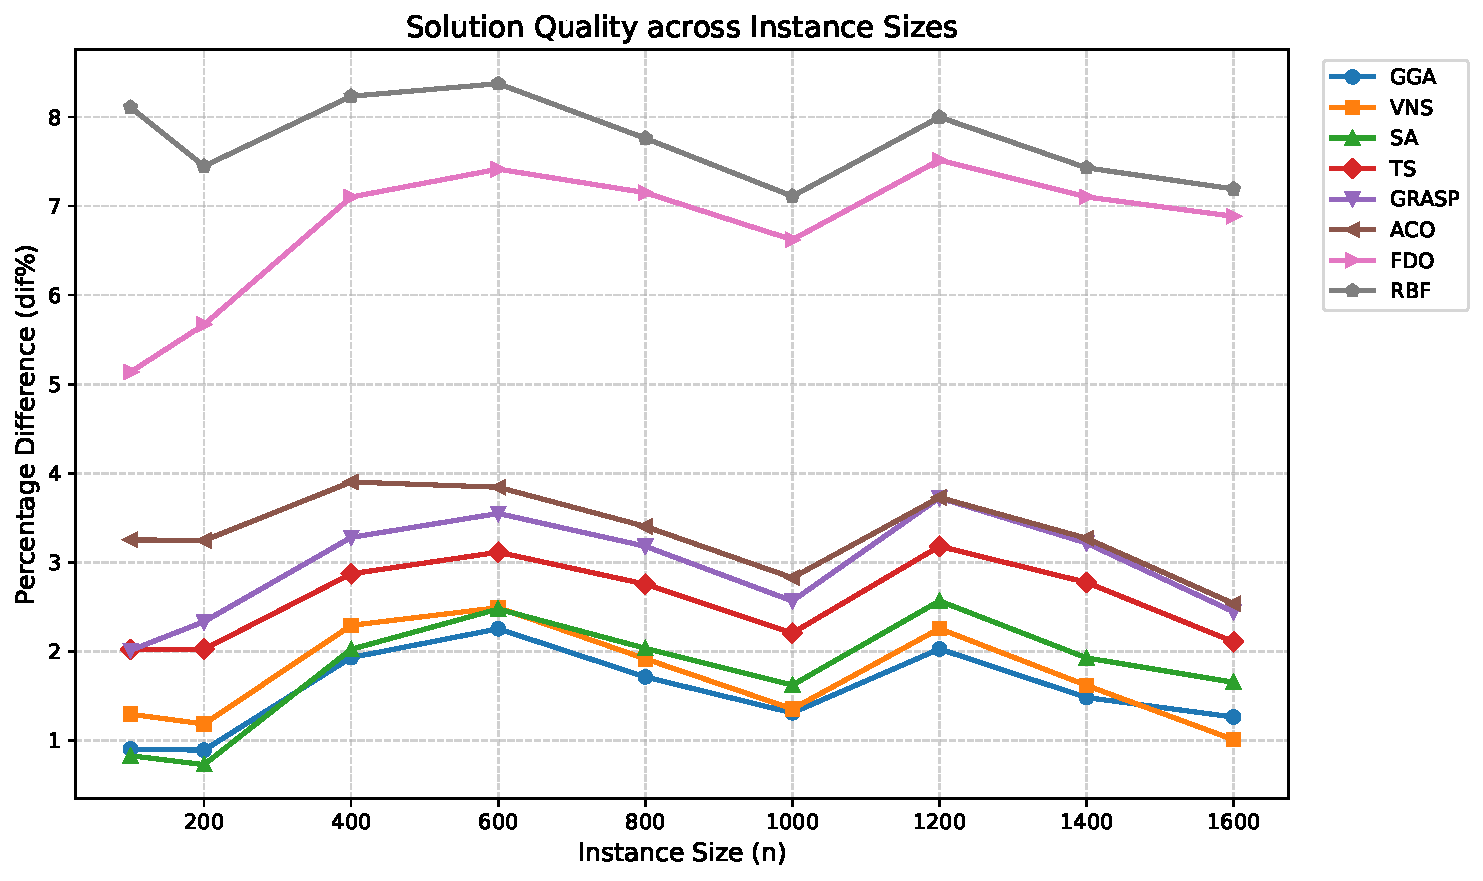
\includegraphics[width=0.85\textwidth]{figures/solution_quality_plot.pdf}
    \caption{Average percentage difference (dif\%) from the theoretical lower bound across varying instance sizes.}
    \label{fig:dif_scaling}
\end{figure}

\begin{figure}[H]
    \centering
    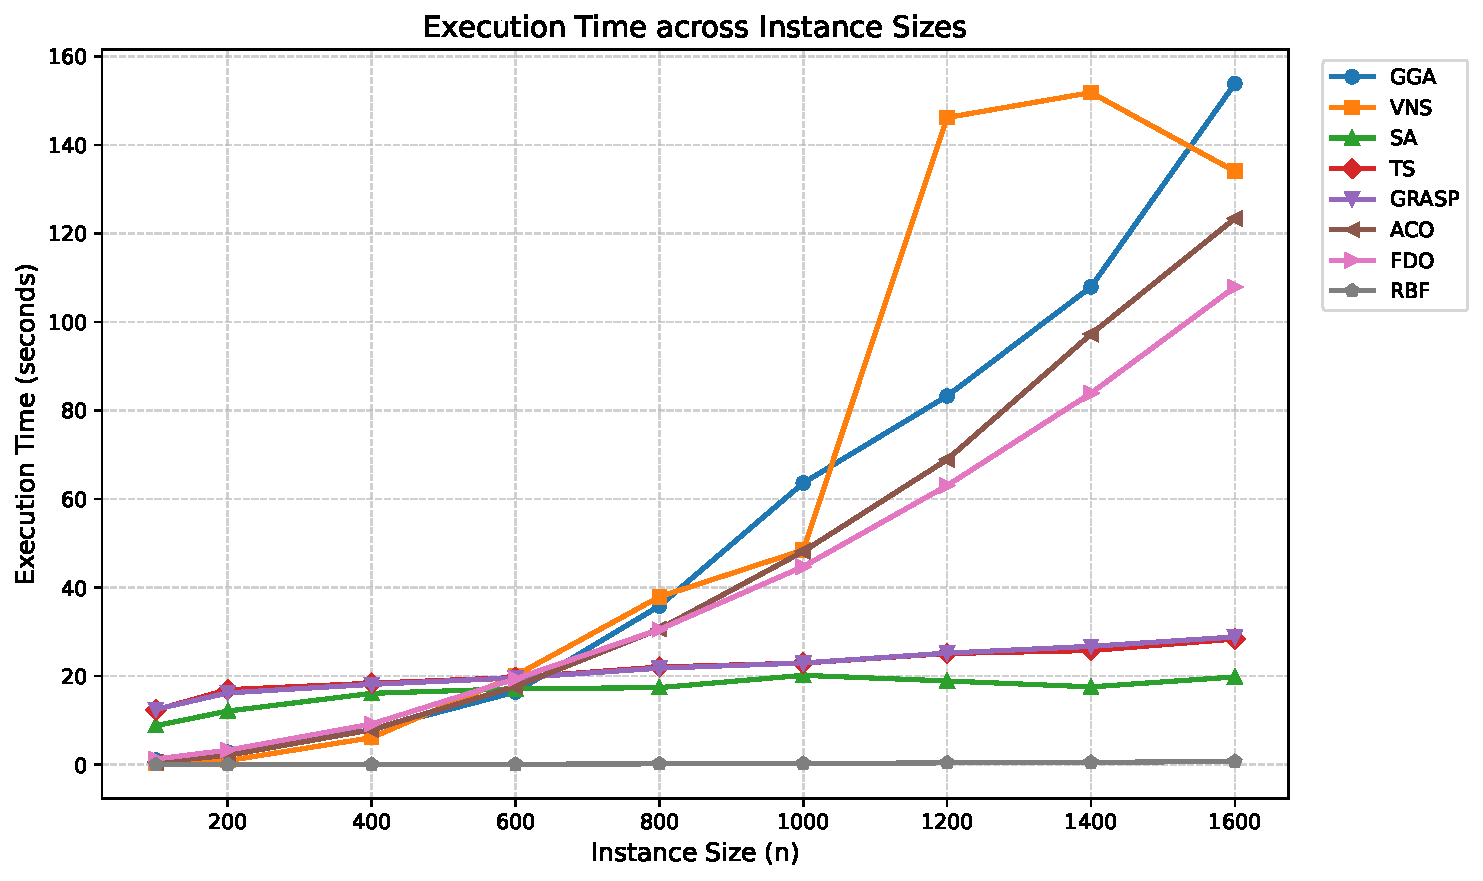
\includegraphics[width=0.85\textwidth]{figures/execution_time_plot.pdf}
    \caption{Average execution time (s) across varying instance sizes.}
    \label{fig:time_scaling}
\end{figure}

\end{document}

